Höfum nú þegar kynnst flutninga- og úthlutunarverkefnum, en þau eru dæmi um netverkefni sem hægt er að leysa með línulegri bestun.
\begin{figure}[h!]
\centering
 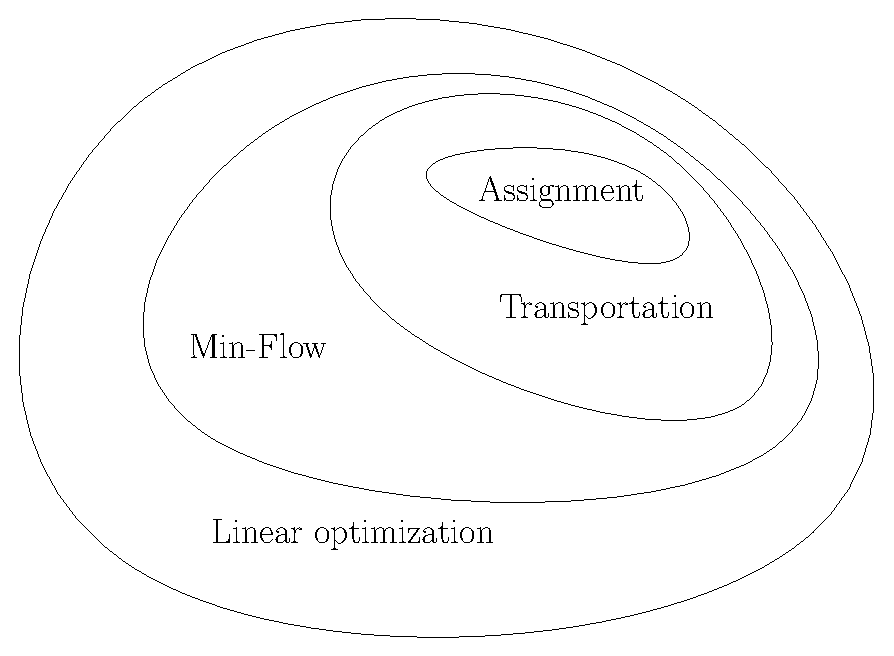
\includegraphics[width=0.6\columnwidth]{figs/types_of_networkproblems.eps}
\end{figure}

Netverkefni eru fjölbreytt bestunarverkefni með margskonar hag\-nýtingu til dæmis:
\begin{itemize}
 \item samgöngukerfum, 
\item fjarskiptum, 
\item fjármálum, 
\item verkefnastjórnun
\item vöru\-stjórnun.
\end{itemize}

\begin{comment}
\begin{itemize}
\item Mikil þróun á aðferðum til að leysa netlíkön.
\item Nokkur sérstök netverkefni:
  \begin{itemize}
  \item stysta leið (e. shortest path),
  \item léttasta spanntré (e. minimum spanning tree)
  \item mesta flæði (e. max flow)
  \item minnsta kostnaðar flæði (e. minimum cost flow)
  \item PERT (program evaluation and review technique) og\\ CPM
  (critical path method).
  \end{itemize}
\end{itemize}
\end{comment}

Mörg hagnýt netverkefni falla undir línulega bestun og má oft finna reiknirit sem eru \emph{sérsniðin} að einstökum tegundum verkefna. En áður en lengra er haldið þarf nokkur hugtök úr \ath{netafræði} (e. graph theory).

\section{Nokkur hugtök úr netafræði}

\begin{description}
 \item[\athsup{Net}{netafræði}] (e. network / graph) er safn af \athsup{hnútum}{netafræði} (e. node) eða punktum og \athsup{leggjum}{netafræði} (e. edges), hver leggur tengir tvo hnúta.
\begin{center} \includegraphics[width=0.37\columnwidth]{figs/network.eps} \end{center}

\begin{center}
\begin{tabular}{|l|lll|}
\hline
Dæmi: & Hnútur & Leggur & Flæði \\ \hline
Vegakerfi & gatnamót & götur  & bílar \\
Flug & flugvellir &  flugleiðir & flugvélar \\
Samskiptakerfi & hnútpunktar & rásir & skeyti\\
Vatnsdreifikerfi & dælur & pípur & vatn \\
Afbrot & krimmar & tengsl krimma & (á ekki við) \\
\hline
\end{tabular}
\end{center}
 \item[\athsup{Stefnt net}{netafræði}] eða örvanet (e. directed network) er net þar sem leggirnir hafa stefnu, þeir eru \athsup{stefndir leggir}{netafræði} eða \athsup{örvar}{netafræði} (e. arc / directed edge). Ef flæði er í báðar áttir, þá er hann óstefndur. %Net sem hefur aðeins stefnda leggi kallast stefnt net.
 \begin{center} \includegraphics[width=0.24\columnwidth]{figs/directed.eps} \end{center}
 \item[\athsup{Leið}{netafræði}] (e. path) er runa af leggjum sem tengir tvo hnúta (örvar sem snúa í rétta átt í örvaneti)
 \begin{center} 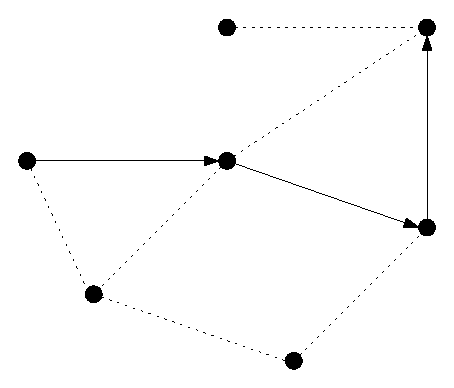
\includegraphics[width=0.27\columnwidth]{figs/path.eps} \end{center}
 \item[\athsup{Rás}{netafræði}] eða hringrás (e. circuit) er leið sem tengir hnút við sjálfan sig (e. cycle / circuit) 
 \begin{center} 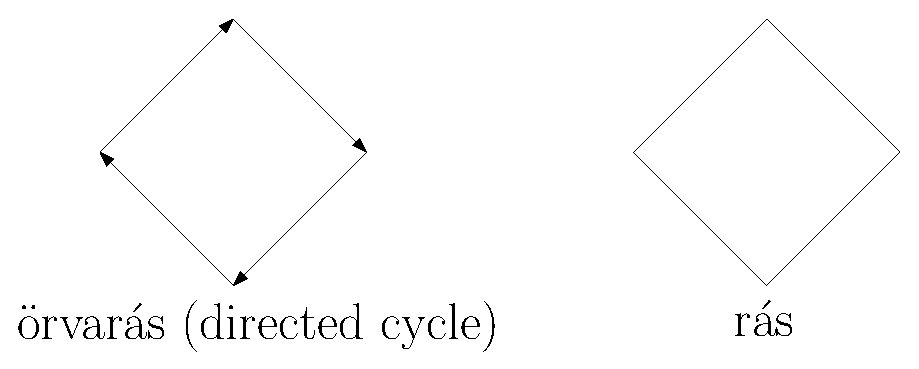
\includegraphics[width=0.6\columnwidth]{figs/cycle.eps} \end{center}
 \item[\athsup{Samhangandi net}{netafræði}] (e. connected graph) er net þar sem til er leið milli sérhverja tveggja punkta í netinu.
 \item[\athsup{Tré}{netafræði}] (e. tree) Tré er samhangandi net sem inniheldur enga hringi, rásalaust net (eða hlutanet).
 \begin{center} \includegraphics[width=0.6\columnwidth]{figs/tree.eps} \end{center}
 \item[\athsup{Spanntré}{netafræði}] (e. spanning tree) í neti er tré sem tengir alla hnúta netsins. %Í neti með $n$ hnúta er alltaf $n-1$ leggur í hverju spanntré.
 \begin{center} 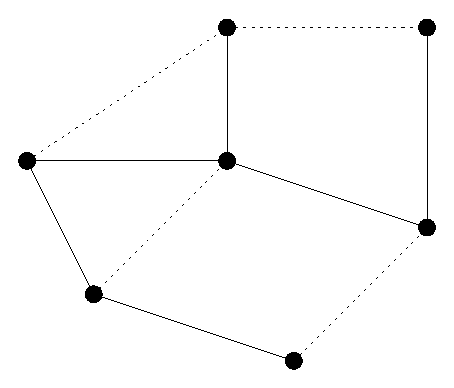
\includegraphics[width=0.3\columnwidth]{figs/spantree.eps} \end{center}
 \item[\athsup{Flæðinet}{netafræði}] (e. flow network) 
 \begin{itemize}
    \item Hverjum legg tengist \athsup{flæði}{netafræði} (oft eru það ákvörðunarbreytur verkefnisins).
    \item Flæðinet hefur \athsup{burðargetu}{netafræði} (e. capacity).
    \item Hnútur með innflæði í net er \athsup{upphafsstaður}{netafræði}, \athsup{upp\-spretta}{netafræði} eða \athsup{lind}{netafræði}.
    \item Þar sem flæðir út úr neti er \athsup{ós}{netafræði}, \athsup{svelgur}{netafræði} eða \athsup{áfangastaður}{netafræði} (e. sink, destination).
    \item Hnútar án inn- eða útflæðis eru \athsup{millihnútar}{netafræði} (e. transshipment node).
  \end{itemize}
 \begin{center} 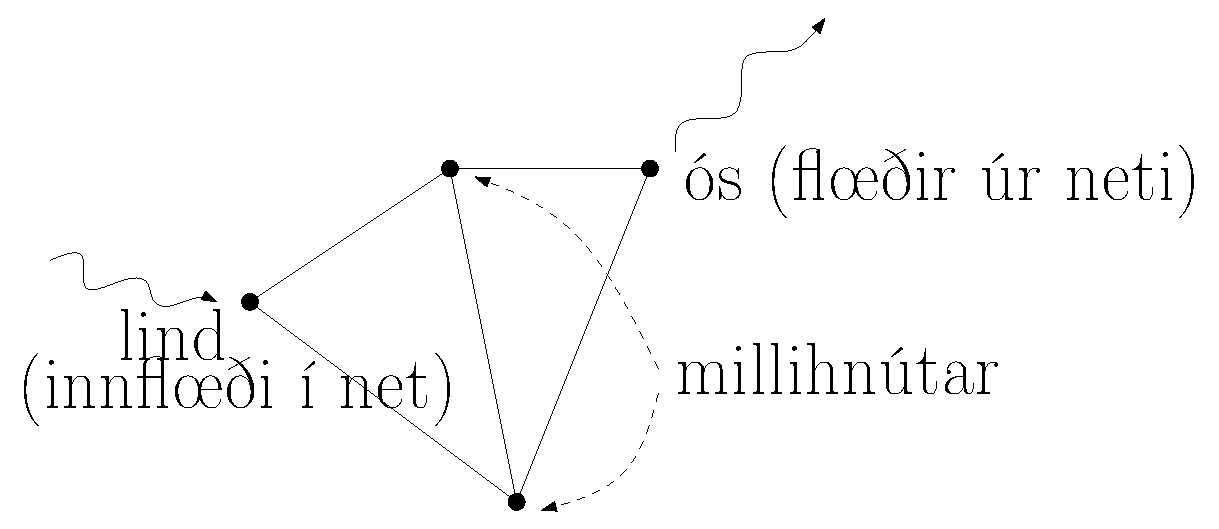
\includegraphics[width=0.6\columnwidth]{figs/flownet.eps}\end{center}
\item{\ath{Stysta leið} (e. shortest path)}
\begin{itemize}
\item Óstefnt, samhangandi net.
\item Upphafspunktur (e. source) og endapunktur (e. sink).
\item Fyrir hvern legg höfum við \emph{fjarlægð} 
\item Markmið: Finna leið sem lágmarkar fjarlægð frá upphafspunkti í endapunkt.
\end{itemize}
\end{description}

\section{Stysta leið}
\begin{daemi}[Seervada garður]\label{daemi:seervada}Finna skal stystu leið á milli upphafsstaðs $O$ og áfangastaðs $T$ gefið:
\begin{center}
  \includegraphics[width=0.7\columnwidth]{figs/seervada.eps}
\end{center}
%\[\begin{array}{lrl}
% \textrm{Stysta leið:} & \min  z = \sum_{i=1}^7 \sum_{j=1}^7 c_{ij}x_{ij}\\
% \textrm{Upphafsstaður:} & \sum_{j=1}^7 x_{Oj} - \sum_{i=1}^7 x_{iO} & =  1\\
% \textrm{Millistaður:} & \sum_{j=1}^7 x_{kj} - \sum_{i=1}^7 x_{ik}  &=  0 \\
% \textrm{Áfangastaður:} & \sum_{j=1}^7 x_{Tj} - \sum_{i=1}^7 x_{iT}  &=  -1
%\end{array}\]
%þar sem $k \in \{A,B,C,D,E\}$, og $x_{ij} \ge 0$ fyrir öll $ i,j \in \{O,A,B,C,D,E,T\}$.
\end{daemi}

Línulegt bestunarverkefni fyrir stystu leið hefur ákvarðanabreytur
\[ x_{ij}=\Big\{\begin{array}{ll} 1 & \textrm{ef leggur }i\to j\textrm{ er á leiðinni}\\ 0 & \textrm{annars}\end{array}\]
Höfum gefna fasta
\begin{eqnarray*}
d_{ij} &=& \textrm{vegalengd milli } i \textrm{ og } j\\
\mathcal{V}&=& \textrm{ mengi hnúta, t.d. } \mathcal{V}=\{O,A,B,C,D,E,T\}\\
\mathcal{E}&=& \textrm{ mengi leggja, t.d. } \mathcal{E}=\{(O,A),(O,C),...,(D,T),(E,T)\}\\
\end{eqnarray*}
Viljum lágmarka 
$$ \min_{\vec{x}} \sum_{(i,j)\in \mathcal{E}} d_{ij}x_{ij} $$
m.t.t. sk.
$$ \underbrace{\overbrace{\sum_{k:(k,i)\in \mathcal{E}}x_{ki}}^{\textrm{innflæði í }i}-\overbrace{\sum_{j:(i,j)\in \mathcal{E}}x_{ij}}^{\textrm{útflæði úr } i}}_{\textrm{nettóflæði}}=\Bigg\{\begin{array}{clc} 1 & \textrm{ef }i=O & \textrm{(lind)}\\-1 & \textrm{ef }i=T& \textrm{(svelgur)}\\0&\textrm{annars}& \textrm{(millinóður)}\end{array}\quad \forall\; i\in \mathcal{V}$$
$$x_{ij}\geq0$$
\begin{aths}Eiginleiki verkefnisins er að í bestu lausn eru öll $x_{ij}=0\vee1$. \end{aths}

\begin{description}
 \item[Afbrigði]\hspace{.1cm}
 \begin{itemize}
  \item Finna minnsta \emph{tíma} sem röð verka tekur.
  \item Finna minnsta \emph{kostnað} við röð verka.
 \end{itemize}
 \item[Notkun]\hspace{.1cm}
 \begin{itemize}
  \item Bestun á samgöngukerfum (t.d. stysta leið milli tveggja staða í borginni).
  \item Tölvunet: stysta leið (um internetið ) frá tölvu $Alice$ til $Bob$.
  \item Stundum má tækla flókin verkefni í aðgerðagreiningu m.þ.a. leysa runu af stystu leiðar verkefnum.
 \end{itemize}

\end{description}



\begin{comment}
\begin{lausn}[á stystu leið dæmis \ref{daemi:seervada} með \athsup{\textsc{matlab}}{Stysta leið}]
Það sem vantar að gera í línulega bestunarverkefninu er að eyða út leggjum sem eru ekki til, t.d. $x_{AC}$. Við getum annað hvort sett $c_{AC} = M$ (stór tala) eða sett $x_{AC} = 0$ (þ.e.a.s. tekið $x_{AC}$ út):
\lstinputlisting{seervada_shortestpath.m}
\begin{center}
  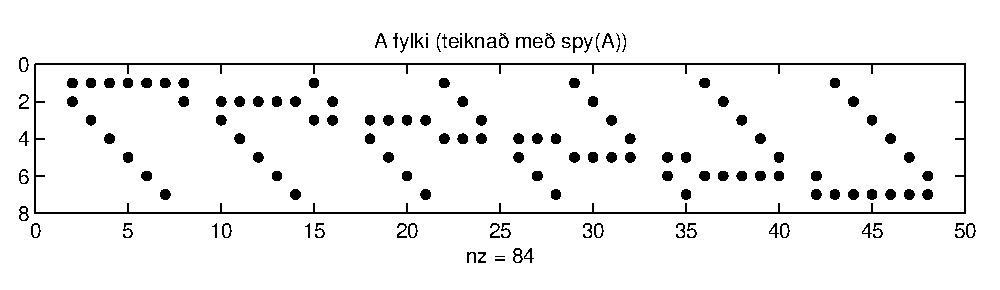
\includegraphics[width=0.7\columnwidth]{figs/seervada-f1.eps}
\end{center}
\end{lausn}
\end{comment}
\newpage
\begin{lausnSYND}[á stystu leið dæmis \ref{daemi:seervada} með \athsub{\textsc{MathProg}}{\texttt{spp.mod}}]\mbox{Almennt} líkan fyrir stystu leið í \textsc{MathProg} er eftirfarandi:
\lstinputlisting[language=awk]{../glpk/spp.mod}
Gagnaskráin fyrir Seervada garðinn er 
\lstinputlisting[language=awk]{../glpk/seervada.dat}\label{seervada.dat}
Keyrum \textsc{glpk} úr skelinni, 
\begin{lstlisting}[language=bash]
hei2@Helga:~/IDN401G/$ glpsol -m spp.mod -d seervada.dat --wcpxlp cplex.skra  
\end{lstlisting}
Lesum úr skelinni (því við notuðum \texttt{printf} skipunina í \texttt{spp.mod}) að leggir í grunni eru 
$$1\leftrightarrow2,\; 2\leftrightarrow3,\; 3\leftrightarrow5,\; 5\leftrightarrow7 \mbox{ með } z^*=13.$$ 
eða með réttum rithætti
$$O\rightarrow A \rightarrow B \rightarrow D \rightarrow T$$ 

Á bak við tjöldin breytti \textsc{glpk} líkanamálinu \textsc{MathProg} í skorður sem það skilur. Hægt er að sjá hvernig þær nákvæmlega litu út með að líta á \textsc{cplex} keyrsluskránna:
\lstinputlisting{../glpk/cplex.skra}
\end{lausnSYND}

\subsection{Reiknirit fyrir stystu leið}
\begin{enumerate}[label=Skref \arabic{*}]
\item \athsup{Leystur hnútur}{Stysta leið} (e. solved node):  Stysta leið í hnútinn frá upphafs\-hnút er þekkt. Í byrjun er upphafshnúturinn eini leysti hnúturinn.
%Byrjið í upphafspunkti. Setjið fjarlægð frá upphafspunkti $=$ núll, þetta kallast merkt fjarlægð, upp\-hafspunkturinn kallast nú leystur hnútur.
\item \label{skref:0} Finnið næsta hnút með:
\begin{enumerate}[label=(\roman{*})]
\item\label{skref1} Skoðið alla óleysta hnúta sem eru tengdir leystum hnút
  (þetta eru kandídatar)
\item\label{skref2} Reiknið fjarlægð að upphafspunkti með því að leggja
fjarlægð í hnút við merkta fjarlægð
\item\label{skref3} Kandídatinn með minnstu fjarlægð frá upphafspunkti verður næsti leysti hnútur (ef jafntefli, leysið þá fyrir báða hnúta)
\end{enumerate}
\item Aftur í \ref{skref:0} uns áfangastaður er leystur hnútur.
\item Stysta leið finnst með því að vinna sig afturábak frá áfangastað.
\end{enumerate}

\begin{lausn}[á stystu leið Seervada úr dæmi \ref{daemi:seervada} með reikniriti]

{\renewcommand{\arraystretch}{1.5} \renewcommand{\tabcolsep}{0.2cm}
{\footnotesize\[
\begin{array}{|p{.5cm}p{1.2cm}cccp{1.3cm}p{1.2cm}|}
\hline
 \textrm{Ítrun } $n$ &
 \textrm{Leystir hnútar }&
 \textrm{\ref{skref:0}\ref{skref1} }&
 \textrm{\ref{skref:0}\ref{skref2} }&
\textrm{\ref{skref:0}\ref{skref3} }& 
 \textrm{Lágmarks fjarlægð} &
 \textrm{Síðasta tenging} \\ 
\hline
1 & O & A & 2 & A & 2 & OA \\ 
\hline
2 & O & C & 4 & C & 4 & OC \\ 
3 & A & B & 2+2=4 & B & 4 & AB \\ 
\hline
 & A & D & 2+7=9 &  &  &  \\ 
4 & B & E & 4+3=7 & E & 7 & BE \\ 
 & C & E & 4+4=8 &  &  &  \\ 
\hline
 & A & D & 2+7=9 &  &  &  \\ 
5 & B & D & 4+4=8 & D & 8 & BD \\ 
 & E & D & 7+1=8 & D & 8 & ED \\ 
\hline
6 & D & T & 8+5=13 & T & 13 & DT \\ 
 & E & T & 7+7=14 &  &  &  \\ 
\hline
\end{array}\]
}}
Allir hnútar eru nú \emph{leystir}. Finnum stystu leið m.þ.a. rekja okkur til baka
$$ T\leftarrow D\leftarrow E \leftarrow B \leftarrow A \leftarrow O$$
eða 
$$ T\leftarrow D\leftarrow B \leftarrow A \leftarrow O$$
með vegalengd $z^*=13$ 
\begin{aths}Fundum tvær \emph{jafn} góðar bestu lausnir. Tökum eftir að \textsc{glpk} fann aðeins seinni lausnina.
\end{aths}


\end{lausn}
\newpage
\subsection{Dijkstra reiknirit}
\lstinputlisting{../matlab/dijkstra.m}

\begin{daemi}[á stystu leið Seervada  úr dæmi \ref{daemi:seervada} með Dijkstra]\hspace{.1cm}
\begin{lstlisting}
>> O=1;A=2;B=3;C=4;D=5;E=6;T=7;
>> c = inf*ones(n,n);
>> c(O,A) = 2; c(A,O) = 2; c(O,B) = 5; c(B,O) = 5; c(O,C) = 4; c(C,O) = 4; c(A,B) = 2; c(B,A) = 2; c(A,D) = 7; c(D,A) = 7; c(B,C) = 1; c(C,B) = 1; c(C,E) = 4; c(E,C) = 4; c(B,E) = 3; c(E,B) = 3; c(B,D) = 4; c(D,B) = 4; c(D,E) = 1; c(E,D) = 1; c(T,E) = 7; c(E,T) = 7; c(T,D) = 5; c(D,T) = 5; 
>> [path, fmin] = shortestpath(c, 1, 7);
tempdist =
     0   Inf   Inf   Inf   Inf   Inf   Inf
tempdist =
   Inf     2     5     4   Inf   Inf   Inf
tempdist =
   Inf   Inf     4     4     9   Inf   Inf
tempdist =
   Inf   Inf   Inf     4     8     7   Inf
tempdist =
   Inf   Inf   Inf   Inf     8     7   Inf
tempdist =
   Inf   Inf   Inf   Inf     8   Inf    14
path =
     1     2     3     5     7
fmin =
    13
>> labels = 'OABCDET'; labels(path)
ans =
OABDT
\end{lstlisting}
\end{daemi}

\section{\ath{Léttasta spanntré}}
\begin{description}
 \item[\ath{Spanntré}  ] Til er leið á milli allra para af hnútum í tréinu.
 \item[\ath{Léttasta spanntré}  (e. minimum spanning tree)] Spanntré þannig að heildar\-lengd leggja er sem minnst.
 \item[Hagnýting]\hspace{.1cm}
\begin{itemize}
 \item Hönnun á samskiptakerftum (ljósleiðaranet)
 \item Samgöngukerfi (lestar, vegir)
 \item Háspennukerfi
 \item Pípukerfi
\end{itemize}
 \item[Inntak í reiknirit]\hspace{.1cm}
 \begin{enumerate}
  \item[$\mathcal{H}$] Safn hnúta
  \item[$\mathcal{L}$] Safn \emph{mögulegra} leggja
  \item[$\mathcal{D}$] Lengd/þyngd leggja í $\mathcal{E}$.
 \end{enumerate}
 \item[Reiknirit]\hspace{.1cm}
 \begin{enumerate}[label=Skref \arabic{*}]
  \item Velja hnút af handahófi 
  \item\label{skref:minspan:aftur} Velja \emph{léttasta legg} sem ekki er þegar kominn í tréið og sem myndar ekki hringrás með leggjunum sem eru þar fyrir. Bætum þessum legg í tréið.
  \item Aftur í \ref{skref:minspan:aftur} þangað til netið inniheldur $n-1$ leggi.
 \end{enumerate}
 \begin{aths}Þetta kallast \ath{gráðugt} (e. greedy) reiknirit. Hægt að stilla upp sem LP -- en ekki alveg eins einfalt.\end{aths}
\end{description}

\begin{lausn}[Léttasta spanntré fyrir Seervada úr dæmi \ref{daemi:seervada}]\hspace{.1cm}
\begin{center}
  \includegraphics[width=0.7\columnwidth]{figs/seervada-tree.eps}
\end{center}
Lægsti heildarkostnaður $2+2+1+3+1+5=14$.
\end{lausn}


\subsection{Samantekt}
\begin{description}
 \item[Stysta leið] Finnur stystu \emph{vegalengd} milli tveggja hnúta.
 \item[Léttasta spanntré] Finnur stystu \emph{heildarvegalengd} milli allra para af hnútum.
\end{description}

\newpage

\section{Hámarksflæði}
Hér er markmiðið að senda sem \ath{mesta flæði} (e. max flow) í gegnum netið. Aðferð
til að leysa þetta verkefni er að:

Viljum finna \ath{hámarksflæði} (e. max flow) frá $A$ til $B$ fyrir eitthvað tiltekið net, t.d.
\begin{center}
  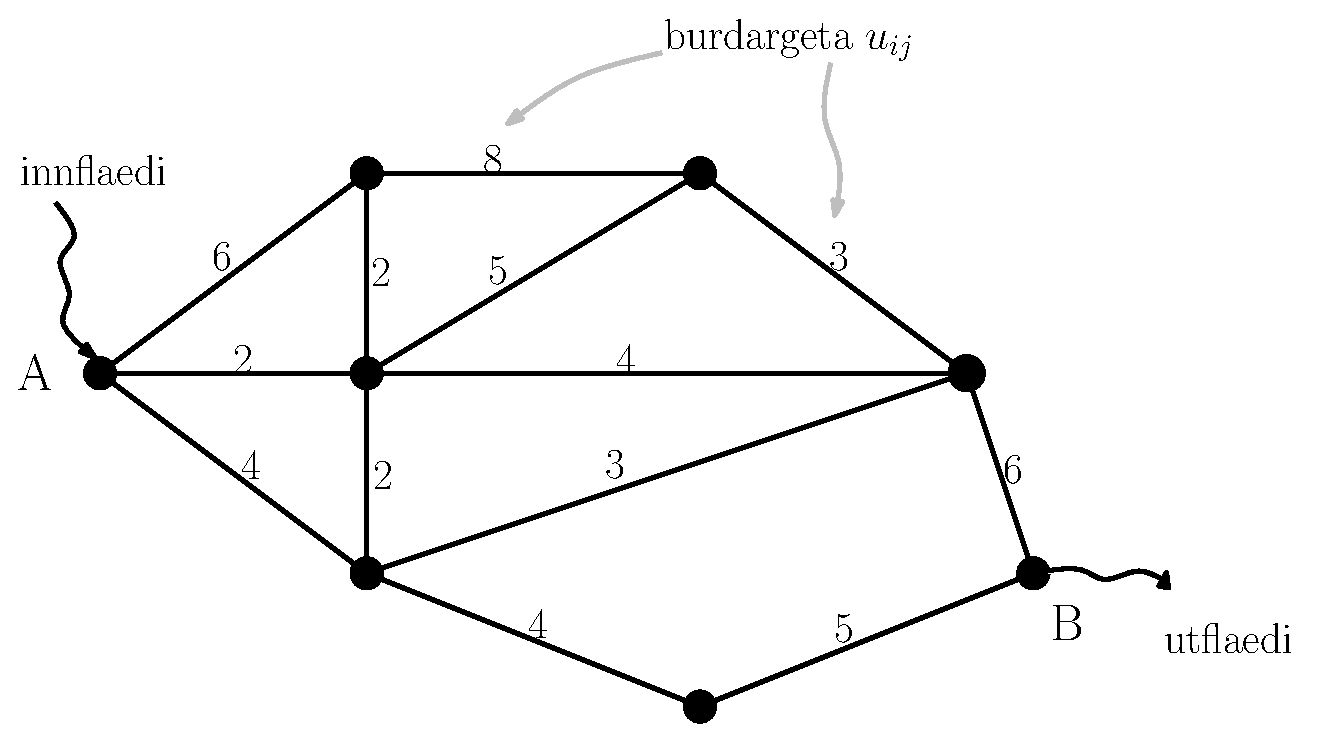
\includegraphics[width=0.7\columnwidth]{figs/maxflow.eps}
\end{center}
Getum gert það m.þ.a.
\begin{itemize}
 \item Nota sérsniðið reiknirit, t.d. \ath{aðferð aukandi vega} (bls. 374--9 í H\&L)
 \item Nota reiknirit fyrir \ath{minnsta kostnaðar flæði} (sjá síðar)
 \item Stilla upp línulegu bestunarlíkani og leysa með Simplex.
\end{itemize}
Fyrir línulegt bestunarlíkan sem hámarkar flæði, látum $\mathcal{H}=\{1,...,n\}$ tákna safn $n$ hnúta og $\mathcal{L}$ tákna safn leggja. Ákvarðanabreytur eru $x_{ij}=$ flæði á legg $i\to j$. Leysum 
$$ \max_{x_{ij}\in\mathcal{L}} d $$ 
m.t.t. sk.
\begin{eqnarray*}
\sum_{i:(i,k)\in\mathcal{L}} x_{ik} - \sum_{j:(k,j)\in\mathcal{L}} x_{kj} &=& 0 \quad \mbox{fyrir }k\in\mathcal{H}\setminus\{1,n\} \\ 
\sum_{j:(1,j)\in\mathcal{L}} x_{1j} &=& s \\ 
\sum_{i:(i,n)\in\mathcal{L}} x_{in} &=& d \\
x_{ij} &\leq& u_{ij} \\
x_{ij}&\geq&0 
\end{eqnarray*}

%\begin{center}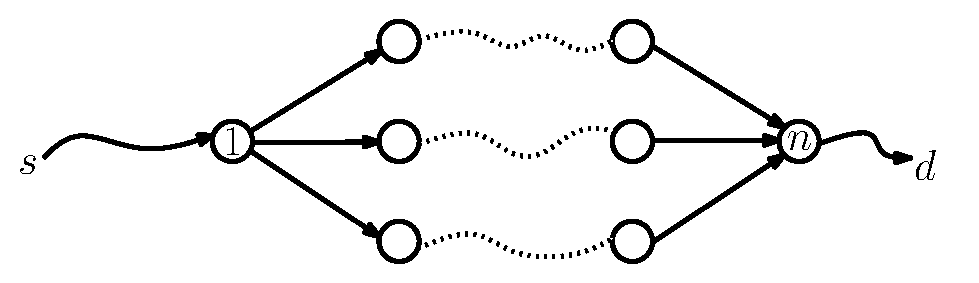
\includegraphics[width=0.75\columnwidth]{figs/maxflow_thm.eps}\end{center}
\begin{samepage}
\begin{aths}\begin{itemize}
\item Fyrstu þrjár skorðurnar hafa í för með sér að $s=d$.
\item Til er afbrigði af hámarksflæði, þ.a. $x_{ij}\geq l_{ij}$.
\end{itemize}
\end{aths}
\end{samepage}
\subsection*{Nokkur dæmi um hagnýtingu}
 \begin{itemize}
  \item Hámarka flæði vatns eða olíu í pípukerfum.
  \item Hámarka flæði faratækja (lestir, bílar) um samgöngumannvirki.
 \item Velja einhverja leið af handahófi í gegnum netið.
\item Finna minnstu burðagetu leiðarinnar og senda það magn í
  gegnum netið. Burðagetan minnkar um þetta magn fyrir þessa leið.
\item Ítrum áfram þangað til engin nýtanleg leið með 
  burðagetu finnst. Þá erum við komin í hámark.
\end{itemize}

\begin{daemi}[Mesta flæði]
Finnum mesta flæði fyrir Seervada (dæmi \ref{daemi:seervada}). 
\end{daemi}

\begin{lausnSYND}[með \athsub{\textsc{MathProg}}{\texttt{maxflow.mod}}]Almennt líkan fyrir mesta flæði er eftirfarandi:
\lstinputlisting[language=Awk]{../glpk/maxflow.mod} 
Höfum gagnaskrá fyrir Seervada garðinn á bls. \pageref{seervada.dat}. 
Keyrum því \textsc{glpk} á eftirfarandi hátt úr skelinni, og lesum bestu lausn beint úr skelinni:
\begin{lstlisting}[language=bash]
hei2@Helga:~/IDN401G/$ glpsol -m maxflow.mod -d seervada.dat
========================================================
Maximum flow from node 1 to node 7 is 11

Starting node   Ending node   Arc capacity   Flow in arc
-------------   -----------   ------------   -----------
            1             2              2             2
            1             4              4             4
            1             3              5             5
            2             5              7             2
            3             5              4             2
            3             6              3             3
            4             6              4             4
            5             7              5             4
            6             7              7             7
========================================================
Model has been successfully processed
\end{lstlisting}
\begin{figure}[h!]
 \begin{center}
  \includegraphics[width=0.7\columnwidth]{figs/seervada_maxflow.eps}
 \end{center}\caption{Hámarksflæði fyrir Seervada garðinn}
\end{figure}
\end{lausnSYND}
\newpage
\begin{daemi}[Nálgun á fylkjum]Viljum nálga eftirfarandi fylki af fleytitölum í heiltölur
\[\begin{array}{ccc}
& & \sum \\
&\begin{bmatrix}
   3.14 & 6.8 & 7.3 \\
   9.6 & 2.4 & 0.7 \\
   3.6 & 1.2 & 6.5 
 \end{bmatrix} & \begin{matrix} 17.24 \\ 12.7 \\ 11.3\end{matrix} \\ 
\sum & \begin{matrix} 16.34 & 10.4 & 14.5\end{matrix}
\end{array}\]
\end{daemi}
\begin{lausn}Setjum upp nálgun fylkisins sem net þ.a. við getum hámarkað flæðið, þ.e.
 \begin{center}
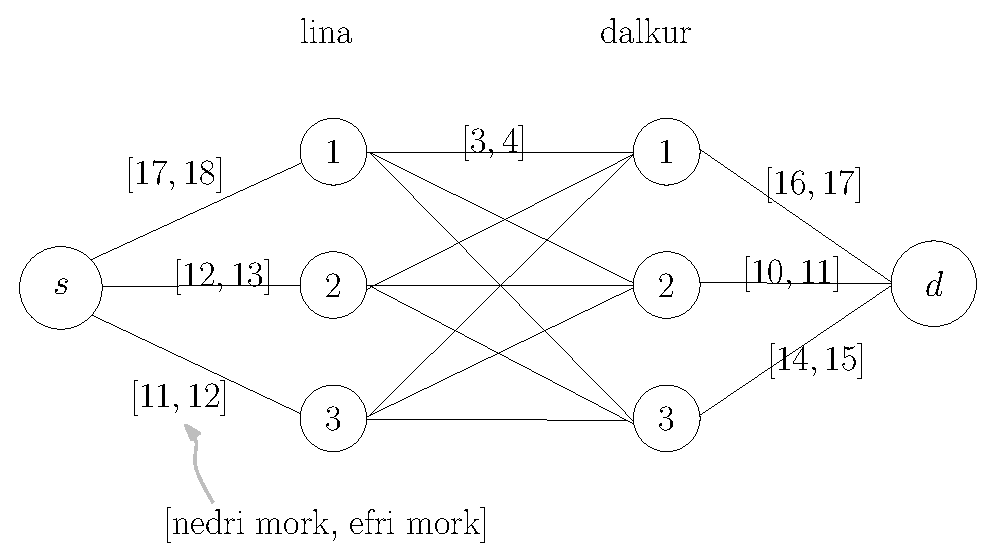
\includegraphics[width=0.75\columnwidth]{figs/maxflow_matrix.eps}
\end{center}
þar sem burðargetan er skorðuð af neðri og efri mörkum á heiltölunálgun gildanna. Besta lausn reynist vera 
\[\begin{array}{ccc}
& & \sum \\
&\begin{bmatrix}
   3 & 7 & 7 \\
   10 & 2 & 1 \\
   3 & 1 & 7 
 \end{bmatrix} & \begin{matrix} 17  \\ 13 \\ 11\end{matrix} \\ 
\sum & \begin{matrix} 16 & 10 & 15\end{matrix}
\end{array}\]
\end{lausn}

\begin{daemi}[Gjaldeyrisbrask]Gengi nokkra gjaldmiðla
\[\begin{array}{c|cccc}\hline 
   &       \mbox{USD} & \mbox{TRY} & \mbox{AED} & \mbox{GBP} \\ \hline 
\mbox{USD} &-& 1.0883 & 3.6732 & 0.7004\\
\mbox{TRY} & 0.5921 &-& 2.1766 & 0.4148\\
\mbox{AED} &0.2722 & 0.4596 &-& 0.1906\\
\mbox{GBP} &1.4298 & 2.4130 & 5.2471 &-\\ \hline 
  \end{array}\]
Sjáum t.d. að $GBP\to TRY\to GBP$ gefur ávöxtun upp á $1.6883\cdot 0.5921=0.9996$ (tap) en $USD\to AED\to GBP\to USD$ gefur $\$0.0010$ í gróða á hvern dollar sem braskað er með.

Hvernig getum við fundið högnunartækifæri (e. arbitrage)?
\end{daemi}
\begin{lausn}
Látum $\mathcal{C}$ tákna mengi gjaldmiðla og $r_{ij}$ tákna gengi á milli gjaldmiðla $i$ og $j$. Ef við byrjum með $USD$ þá getum við \emph{leitað} að högnun m.þ.a. leysa
$$ \max d$$
m.t.t. sk.
\begin{eqnarray*}
 \sum_{j\in\mathcal{C},\;j\neq i} x_{ij}-\sum_{j\in\mathcal{C},\;j\neq i} x_{ji}r_{ji} = 0\quad\forall\;i\in\mathcal{C}\setminus\{USD\} \\
 f+\sum_{j\in\mathcal{C}\setminus\{USD\}} x_{USD,j}-\sum_{j\in\mathcal{C}\setminus\{USD\}} x_{j,USD}r_{j,USD}=1\\
f\leq 2,\quad x_{ij}\geq 0
\end{eqnarray*}
Sjáum að þetta er náskylt mesta flæðis verkefninu.

Besta lausn gefur ávöxtun $1.00143$ á dollar ef $USD\to GBP\to USD$ þ.e.a.s. við þurfum $\$683$ til þess að græða $\$1$.
\begin{aths}Gerðum ekki ráð fyrir þóknun.\end{aths}

\end{lausn}



\section{Flæði lægsta kostnaðar}
\ath{Flæði lægsta kostnaðar} (e. minimum cost flow) er nokkuð almennt verkefni, undir það fall m.a. stysta leið, mesta flæði og flutningsverkefni (sjá nánar 386--9 í H\&L). Til er hagkvæmt reiknirit sem kallast \ath{Netsimplex aðferðin}.

\subsection{Netsimplex aðferðin}
\ath{Netsimplex-aðferðin} er sérsniðin að minnsta kostnaðar flæðisverkefni. Hún byrjar á einhverri gjaldgengri spanntréslausn og rekur sig á milli slíkra lausna með  því að skipta út einum legg í hverju skrefi  þar til komið er í bestu lausn.
\begin{description}
 \item[Ákvörðunarbreytur]$x_{ij} = $ flæði í gegnum legg $i \rightarrow j$
 \item[Gögn]\hspace{.1cm}
\begin{itemize}
\item $c_{ij}$ kostnaður við flæði á legg $i\to j$
\item $u_{ij}$ \ath{burðargeta leggs} (e. arc capacity) fyrir legg $i\to j$
\item $b_i$ er heildarflæði í hnút $i$
\begin{itemize}
\item $b_i > 0$ ef hnútur $i$ er lind
\item $b_i < 0$ ef hnútur $i$ er svelgur
\item $b_i = 0$ ef hnútur $i$ er millihnútur
\end{itemize}
\end{itemize}
\end{description}
Línulegt verkefni sem lágmarkar heildarkostnað, summan er aðeins tekin yfir leggi sem eru til staðar:
$$\min_\vec{x} ~~  Z = \sum_{i=1}^{n}\sum_{j=1}^{n}c_{ij}x_{ij}$$
skorður fyrir hvern hnút $i\in\mathcal{H}$
$$\sum_{j\in \deg^-(i)} x_{ij}-\sum_{j\in\deg^+(i)}^n x_{ji}=b_i$$
og efra mark á ákvörðunarbreytum
$$0 \le x_{ij} \le u_{ij}$$

\begin{samepage}\begin{aths}Skilyrði fyrir að verkefnið hafi löglega lausn er \mbox{$\sum_{i\in\mathcal{H}} b_i = 0$}.
Ef $b_i$ og $u_{ij}$ eru allar heiltölur þá verða ákv.breyturnar ($\vec{x}^*$) líka heiltölur.
\end{aths}\end{samepage}

\begin{daemi}Höfum gefið eftirfarandi net:
\begin{center}
\includegraphics[width=0.9\columnwidth]{figs/netsimplex.eps} 
\end{center}
\end{daemi}


\begin{lausn}Beitum netsimplex-aðferðinni:
\begin{comment}
\begin{enumerate}[label=(\arabic{*})]
 \item Fyrsta grunnlausn 
  \begin{center}
  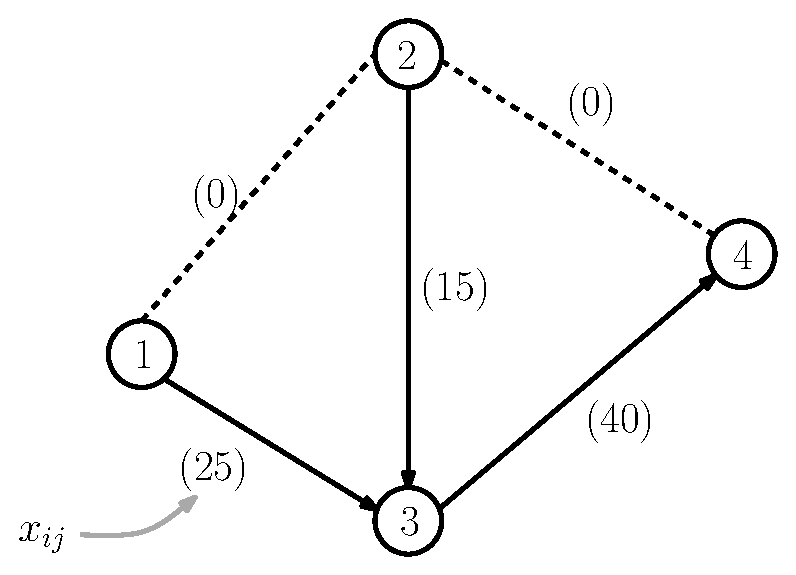
\includegraphics[width=0.6\columnwidth]{figs/netsimplexstart.eps}
  \end{center}
  \item %Ítrun 1
    Ef ör $1\to 2$ er bætt í tréð myndast hringrás og ef flæðið eftir $1\to 2$ er aukið um $\theta$ (það er 0) og flæði eftir öðrum örvum er aukið eða minnkað um $\theta$ og þá breytist $z$ um \[\Delta z = \sum_{(i,j)\in\mbox{hringrás}}c_{ij}(\pm\theta)=2\theta+8\theta-7\theta = 3\theta\quad\Rightarrow\;\frac{\partial z}{\partial \theta}=3\]
    Ef ör $2\to 4$ bætt við er $\frac{\partial z}{\partial \theta}=3-6-8=-11$. \linebreak 
    Nýr grunnur og lausn:
    \begin{center}
    \includegraphics[width=0.5\columnwidth]{figs/netsimplex-1.eps}
    \end{center}
    bætum ekki við ör $2\to 3$ því þá förum við aftur í upphafslausn.
  \item %Ítrun 2
Ör $1\to 2$ gefur $\Delta z = 2+3-6-7=-8$ og nýja flæðið breytist:\linebreak
\begin{center}
  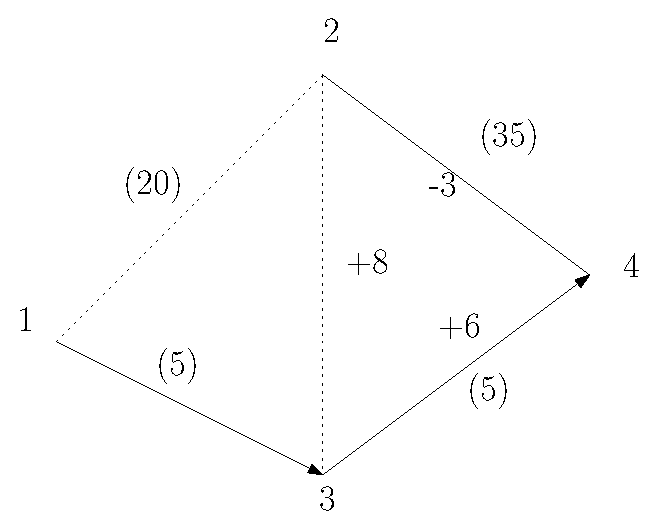
\includegraphics[width=0.5\columnwidth]{figs/netsimplex-2.eps}
\end{center}
Athugið að örin $1\to 2$ sem er í efri mörkum telst ekki vera í grunni. Hérna notum við \emph{upper bound} aðferðina og
skiptum út $x_{12}$ með \mbox{$u_{12} - y_{12}$} þar sem $0\le y_{12} \le u_{12}$ (lesið kafla 7.3 í H\&L).
\item %Ítrun 3
Ef flæðið eftir $2\rightarrow 3$ er aukið: $\Delta z = +8\theta+6\theta-3\theta = 11\theta$\linebreak
Ef flæðið eftir $1\rightarrow 2$ er minnkað um $\theta$: $\Delta z = -c_{12}\theta -c_{24}\theta+c_{34}\theta+c_{13}\theta=-2\theta-3\theta+6\theta+7\theta = 8\theta$ (þetta síðasta var í raun óþarfi  því við vorum  að bæta inn flæði eftir $1\rightarrow 2$ í 2. ítrun, en sýnir hvernig reiknað er ef ör sem er í efri mörkum  kæmi í grunn. \linebreak
Bæði $\Delta z >0$ svo besta lausn er fundin.
\end{enumerate}
\end{comment}
\end{lausn}








\newpage
\begin{daemi}[Minnsta kostnaðar flæði í \textsc{MathProg}]\hspace{.1cm}
\lstinputlisting{../glpk/mincostflow.mod}
\end{daemi}



\subsection{Samband minnsta kostnaðar og mesta flæðis}
Hægt er að nota \ath{min cost flow} lausnaraðferðir til þess að leysa \ath{max flow} verkefni. Hugsum okkur að við höfum max flow verkefni með eina lind (e. source), eina ós (e. sink) og nokkra hnúta (e. nodes) ásamt hámarksburðargetu leggja. Til að breyta þessu verkefni yfir í min cost flow verkefni þarf einungis að breyta þrennu:
\begin{enumerate}
\item Látum kostnaðinn $c_{ij}=0$ fyrir öll $i,j$ þ.e. setjum kostnað sérhvers leggs jafnt og núll.
\item Veljum nægilega stórt $\hat{F}$, sem á að tákna öruggt efra mark gjaldgengs flæðis í gegnum netið. Þ.e. setjum $\hat{F}$ á lindina og $-\hat{F}$ á ósina.
\item Búum til nýjan legg milli lindar og ósar, setjum á hann ótakmarkaða burðargetu og stóran kostnað $M$.
\end{enumerate}

Tökum eftir að lágmörkun kostnaðar þess verkefnis jafngildir að hámarka flæði í gegnum upphaflega netið. Því vissulega viljum við lágmarka flæðið sem fer í gegnum nýja legginn sem hefur mikinn kostnað, sem gerist einmitt þegar sent er sem mest flæði í gegnum upphaflega netið.



\section{\ath{Critical Path Method} (CPM)}
\begin{daemi}[Verkefnastjórnun] Lágmarka á tíma sem tekur að byggja  hús (sjá töflu bls. 400 og mynd bls. 402). 
Viljum vinna verkið á 40 vikum. Hvernig er hagkvæmast að gera það?
\end{daemi}
\begin{lausn}
Getum fundið sex mismunandi vegi í gegnum netið:
{\footnotesize
\begin{verbatim}
    * Start A B C D G H M Finish       Lengd: 40 vikur
    * Start A B C E H M Finish         Lengd: 31 vikur
    * Start A B C E F J K N Finish     Lengd: 43 vikur
    * Start A B C E F J L N Finish     Lengd: 44 vikur
    * Start A B C I J K N Finish       Lengd: 41 vika
    * Start A B C I J L N Finish       Lengd: 42 vikur
\end{verbatim}}
Sú lengsta tekur 44 vikur. Þetta er stysti tíminn sem verkið getur tekið (kostn. 4.55 milljónir).
\begin{quote} Verk á þessari leið eru \emph{flöskuhálsar} -- mikilvægt að þeim seinki ekki.
%Til að stytta tímann þurfum við að skoða þann veg og hvaða verkþátt er hægt að stytta. 
\end{quote}
Oft má flýta einstökum verkþáttum m.þ.a. auka við mannskap, vélar, tæki, meiri yfirvinnu o.s.frv. Af þessu hlýst viðbótarkostnaður. Ef öllum verk\-þáttum er flýtt einsog mögulegt er þá tekur verkið 28 vikur og kostnaður er 6.15 milljónir. 

Setjum upp línulegt bestunarverkefni:
\begin{description}
 \item[Ákvarðanabreytur]\hspace{.1cm}
\begin{description}
\item[$x_j$] tími sem verk $j$ er stytt um.
\item[$y_j$] upphafstími verks $j$.
\end{description}
\item[Gefið]\hspace{.1cm}
\begin{description}
 \item[$t_j$] tími sem tekur að vinna verk $j$.
 \item[$c_j$] kostnaður við að \emph{krassa} verki.
\end{description}
\end{description}
Vandamálið snýst því um að lágmarka 
$$ \min_{\vec{x},\vec{y}} z= \sum_{j\in\mathcal{H}} c_jx_j $$
m.t.t. sk.
\begin{eqnarray*}
 y_j\geq y_i+t_i-x_i &&\mbox{fyrir öll verk } i \mbox{ sem eru undanfarar }j\\
 y_{finish}\leq 40 \\ y_i\geq0 && 0\leq x_j\leq x_j^{\max} 
\end{eqnarray*}
\end{lausn}

